\documentclass[12pt, letterpaper]{article}
\usepackage{graphicx}
\graphicspath{{images/}}

\title{Homework 1}
\author{Alex Bryan}
\date{January 26, 2024}

\begin{document}
\maketitle

\section{Problem 1}

Suppose that three teams are engaged in a tug-of-war. Each of the three teams is pulling on a tire, as pictured in Figure 1.

\begin{figure}[hpt]
    \centering
    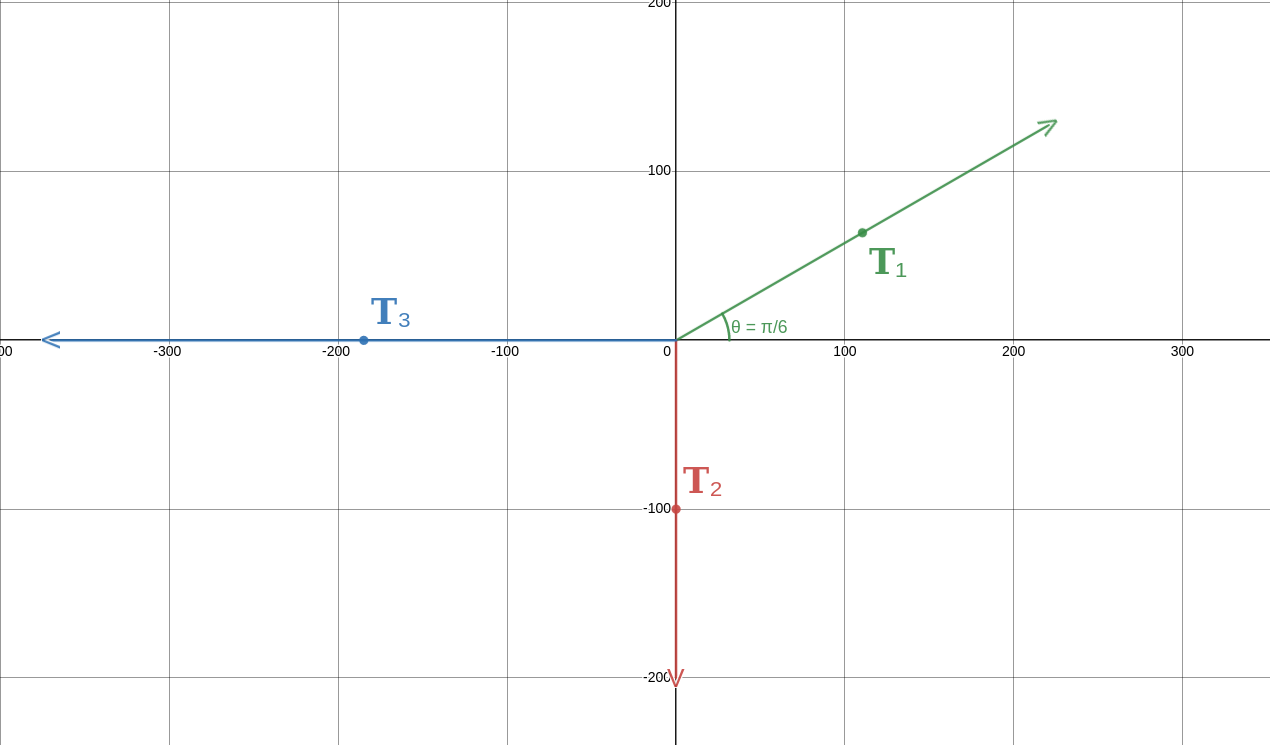
\includegraphics[width=0.75\textwidth]{tug}
    \caption{Tug-Of-War between three teams}\label{tug.png}
\end{figure}

\subsection{Part a}

If team 1, team 2, and team 3 are pulling with a force of 255 N (Newtons), 200 N, and 370
N, find the net force vector acting on the tire (assuming no other forces are in play).

Firstly, the forces exerted on the tire by team 1, team 2, and team 3 are all vectors. By considering the tire as the origin, these vectors can be expressed in standard position.

If team 1 is pulling with a force of 255N at an angle 30 degrees North of East (\( \frac{\pi}{6} \) radians), then the endpoint of Team 1 can be calculated using the formula
\( \langle |\textbf{T}_1|\cos(\theta), |\textbf{T}_1|\sin(\theta) \rangle \), where \( |\textbf{T}_1| = 255 \) and \( \theta = \frac{\pi}{6} \).


\[ \textbf{T_{1}} = \langle 255\cos(\frac{\pi}{6}), 255\sin(\frac{\pi}{6}) \rangle \] 

\newline

\[ \textbf{T_{2}} = \langle 0, -200 \rangle \] 

\newline

\[ \textbf{T_{3}} = \langle -370, 0 \rangle \] 

\newline

To find the net force vector \textbf{U},

\end{document}